\documentclass[eikonal.tex]{subfiles}

\begin{document}

\begin{figure}[t]
  \centering
  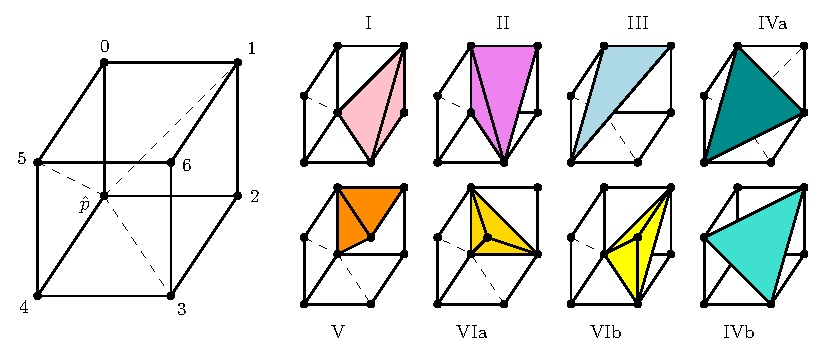
\includegraphics{simplex-groups.eps}
  \caption{Numbering scheme for an update octant. The node $\hat{p}$
    is having its value updated. The diagonally opposite node is the
    sixth (last) node, with the other six nodes numbered 0--5
    cyclically.}\label{fig:octant-numbering}
\end{figure}
  
\begin{figure}[t]
  \centering
  \begin{tabular}{c|cccccc|cccccc|cccccc|cc}
    0 & $\bullet$ & & & & $\bullet$ & $\bullet$ & $\bullet$ & & & $\bullet$ & & $\bullet$ & $\bullet$ & & $\bullet$ & & & $\bullet$ & $\bullet$ & \\
    1 & $\bullet$ & $\bullet$ & & & & $\bullet$ & $\bullet$ & $\bullet$ & & & $\bullet$ & & $\bullet$ & $\bullet$ & & $\bullet$ & & & & $\bullet$ \\
    2 & $\bullet$ & $\bullet$ & $\bullet$ & & & & & $\bullet$ & $\bullet$ & & & $\bullet$ & & $\bullet$ & $\bullet$ & & $\bullet$ & & $\bullet$ & \\
    3 & & $\bullet$ & $\bullet$ & $\bullet$ & & & $\bullet$ & & $\bullet$ & $\bullet$ & & & & & $\bullet$ & $\bullet$ & & $\bullet$ & & $\bullet$ \\
    4 & & & $\bullet$ & $\bullet$ & $\bullet$ & & & $\bullet$ & & $\bullet$ & $\bullet$ & & $\bullet$ & & & $\bullet$ & $\bullet$ & & $\bullet$ & \\
    5 & & & & $\bullet$ & $\bullet$ & $\bullet$ & & & $\bullet$ & & $\bullet$ & $\bullet$ & & $\bullet$ & & & $\bullet$ & $\bullet$ & & $\bullet$ \\
    \multicolumn{1}{c}{} & \multicolumn{6}{c}{I} & \multicolumn{6}{c}{II} & \multicolumn{6}{c}{III} & \multicolumn{2}{c}{IV}
  \end{tabular}
  \caption{Enumeration of tetrahedra that do not involve the sixth
    node. These are OLIM18's only tetrahedra, and are common to
    OLIM26. The tetrahedra (0, 1, 2), (2, 3, 4), and (4, 5, 0) in
    group I are degenerate and can be omitted; the other three must be
    included. All of the tetrahedra in groups II and III have a
    pairwise distance that is greater than $h \sqrt{2}$ and can be
    omitted. The remaining tetrahedra in group IV must be
    included.}\label{fig:olim18-tetrahedra}
  \vspace{1em}
  \begin{tabular}{c|cccccc|cccccc|ccc}
    0 & $\bullet$ & & & & & $\bullet$ & $\bullet$ & & & & $\bullet$ & & $\bullet$ & & \\
    1 & $\bullet$ & $\bullet$ & & & & & & $\bullet$ & & & & $\bullet$ & & $\bullet$ & \\
    2 & & $\bullet$ & $\bullet$ & & & & $\bullet$ & & $\bullet$ & & & & & & $\bullet$ \\
    3 & & & $\bullet$ & $\bullet$ & & & & $\bullet$ & & $\bullet$ & & & $\bullet$ & & \\
    4 & & & & $\bullet$ & $\bullet$ & & & & $\bullet$ & & $\bullet$ & & & $\bullet$ & \\
    5 & & & & & $\bullet$ & $\bullet$ & & & & $\bullet$ & & $\bullet$ & & & $\bullet$ \\
    6 & $\bullet$ & $\bullet$ & $\bullet$ & $\bullet$ & $\bullet$ & $\bullet$ & $\bullet$ & $\bullet$ & $\bullet$ & $\bullet$ & $\bullet$ & $\bullet$ & $\bullet$ & $\bullet$ & $\bullet$ \\
    \multicolumn{1}{c}{} & \multicolumn{6}{c}{V} & \multicolumn{6}{c}{VI} & \multicolumn{3}{c}{VII}
  \end{tabular}
  \caption{Enumeration of tetrahedra involving the node diagonally
    opposite $\hat{p}$---i.e., OLIM26-only tetrahedra. All of the
    tetrahedra in groups V and VI have pairwise distances no greater
    than $h \sqrt{2}$ and must be included. The tetrahedra in group
    VII are all degenerate and can be
    omitted.}\label{fig:olim26-tetrahedra}
  \vspace{1em}
\end{figure}

\end{document}

%%% Local Variables:
%%% mode: latex
%%% TeX-master: "sisc-eikonal"
%%% End:
